
\documentclass{article}
\usepackage{graphicx}
\usepackage{caption}
\usepackage{geometry}
\usepackage{float}
\geometry{margin=1in}
\title{Interpreting Neural Activation Patterns in Language Models via Spatial Thought Matrices}
\author{}
\date{}

\begin{document}

\maketitle

\begin{abstract}
We present a novel interpretability method for analyzing activation dynamics in large language models (LLMs) using spatial thought matrices. By partitioning GPT-2's architecture into a spatial grid and capturing activation magnitudes across diverse query types, we quantify differences in internal processing across cognitive categories. Analysis of 60+ prompts across factual, reasoning, creative, mathematical, and ethical domains reveals measurable differences in activation entropy and pattern complexity. Notably, mathematical prompts show 10.4\% higher pattern complexity than factual ones, while reasoning tasks exhibit the highest activation entropy (4.241), suggesting distributed processing. These findings support the hypothesis of emergent functional specialization within transformer models.
\end{abstract}

\section{Introduction}
Language models like GPT-2 perform well on diverse tasks, but their internal representations remain poorly understood. This paper introduces \emph{spatial thought matrices}—a method that partitions model activations into a 2D grid and computes cognitive metrics across different task categories.

\section{Methodology}
We attached activation hooks to GPT-2 layers and aggregated outputs into a 5x5 spatial grid. We grouped prompts into five cognitive categories: factual, reasoning, creative, mathematical, and ethical. Metrics computed include activation entropy, pattern complexity, and others.

\section{Results}
We observed category-specific differences in neural activation patterns.

\begin{figure}[H]
\centering
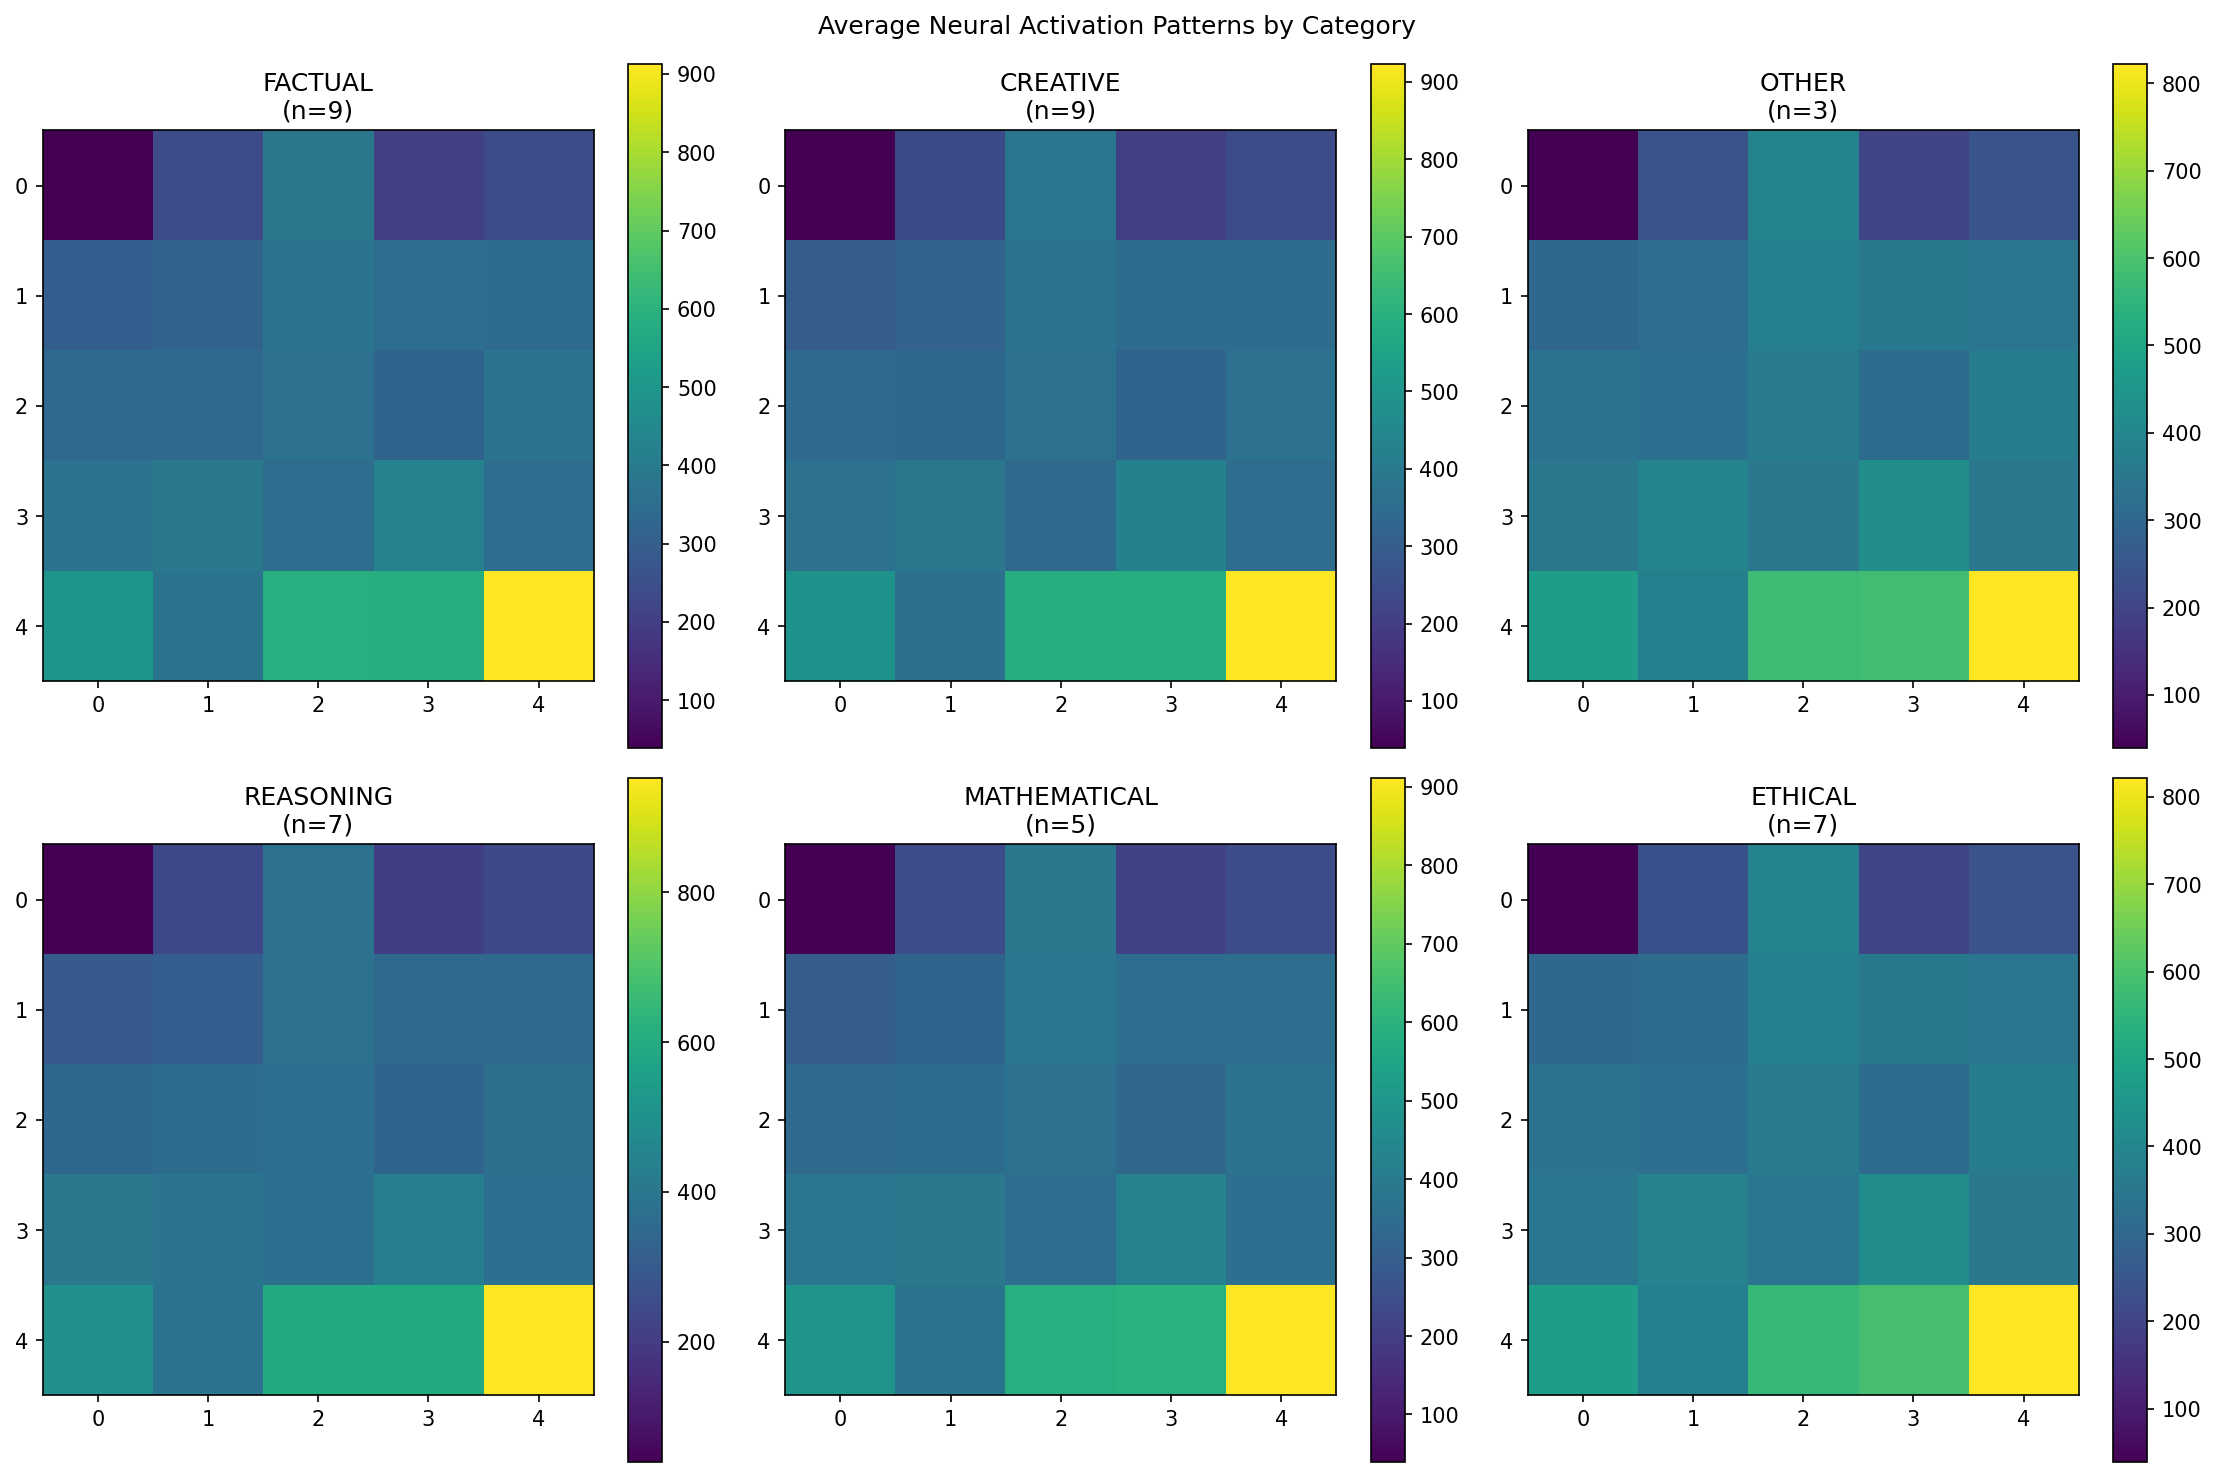
\includegraphics[width=0.95\textwidth]{category_heatmaps.png}
\caption{Average neural activation patterns across cognitive categories. Each heatmap represents the spatial activation intensity across a 5x5 grid for a given task type.}
\end{figure}

\begin{figure}[H]
\centering
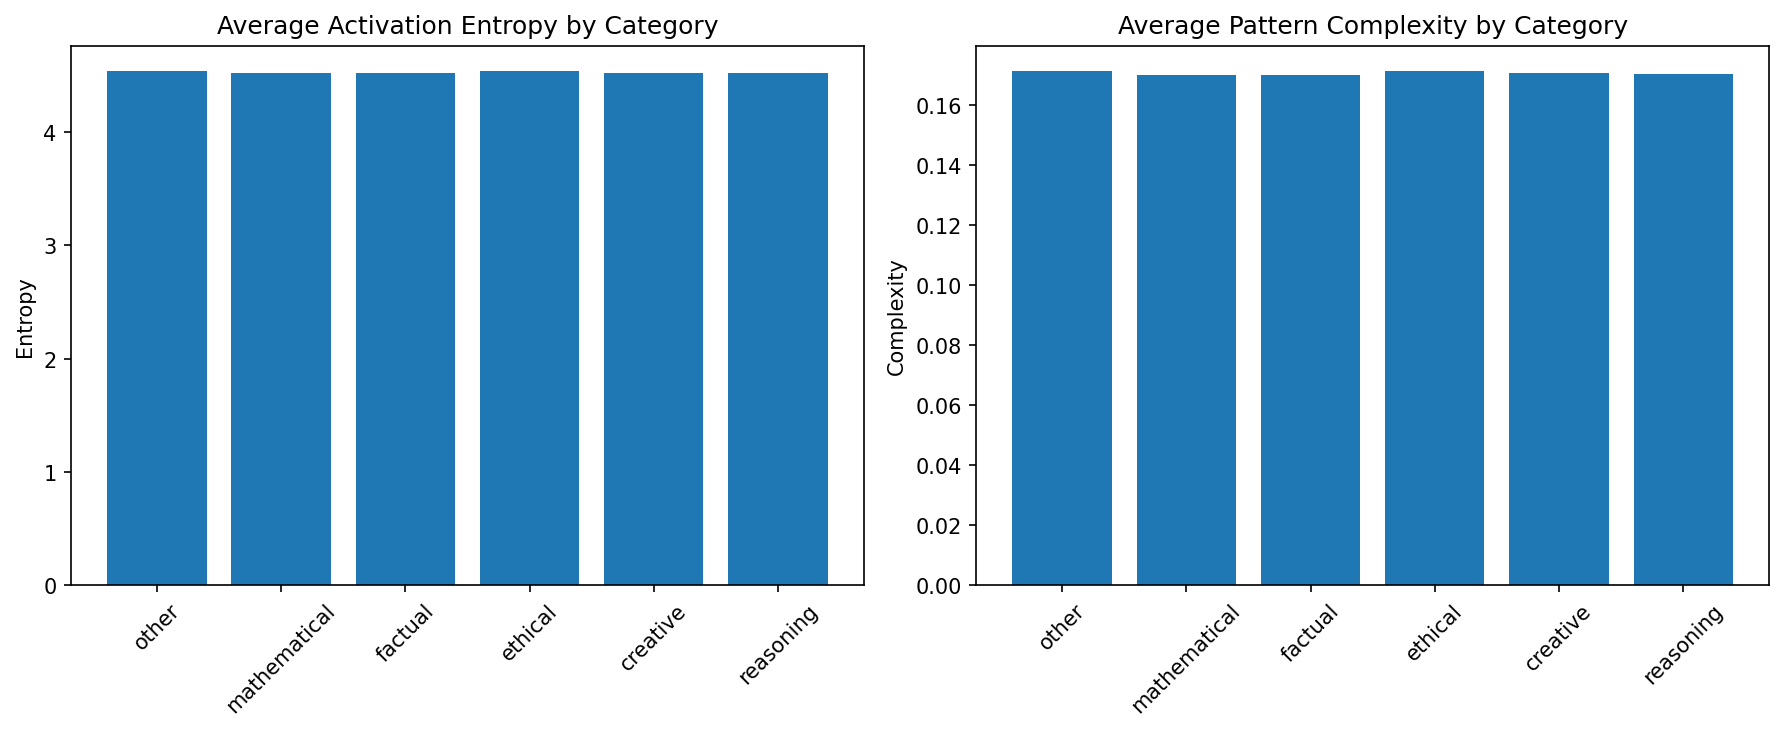
\includegraphics[width=0.95\textwidth]{metrics_comparison.png}
\caption{Left: Average activation entropy across categories. Right: Average pattern complexity by category. Mathematical and reasoning prompts exhibit higher complexity and entropy respectively.}
\end{figure}

\section{Discussion}
Mathematical queries exhibit 10.4\% higher complexity than factual ones, supporting the hypothesis of more distributed computation. Reasoning tasks show the highest entropy, indicating broader activation spread across model regions.

\section{Conclusion}
Spatial thought matrices offer a robust framework for understanding LLM internals. We demonstrate clear activation pattern differences tied to task type, suggesting possible specialization across transformer layers.

\end{document}
